\documentclass[boxes]{beamer}
%\usepackage[bookmarks=false,hidelinks,pdfpagelabels=false,hyperfootnotes=false,hyperindex=false,pageanchor=false,draft]{hyperref}
\usepackage{cite}
\usepackage{amsmath}
\usepackage{amsfonts}
\interdisplaylinepenalty=2500
\usepackage{array}
\usepackage{mdwmath}
\usepackage{mdwtab}
\usepackage{stfloats}
\usepackage{url}
\usepackage{multirow}
\usepackage{graphicx, tikz, pgfplots}
\pgfplotsset{compat=1.16}
\usetikzlibrary{calc}
\usetikzlibrary{pgfplots.groupplots}
\usetikzlibrary{plotmarks}

\usepackage{attachfile}

\usepackage{xargs}
\usepackage{filecontents}
%%\usepackage{datatool-pgfmath}
\usepackage{datatool}
\DTLsetseparator{ }
\usepackage{xstring}
\usepackage{ifthen}

\makeatletter

\makeatother

%for printing, though this current paper should be black and white
\selectcolormodel{rgb}

%fit the plots with the page margins
\def\plotWidth{8.5cm}


% correct bad hyphenation here
%\hyphenation{op-tical net-works semi-conduc-tor}


\definecolor{SynascPurple}{RGB}{130,30,250}
\setbeamercolor{title}{fg=SynascPurple}
\setbeamercolor{frametitle}{fg=SynascPurple}
\setbeamercolor{structure}{fg=SynascPurple}

\setbeamertemplate{navigation symbols}{}%remove navigation symbols

\begin{document}


\title{Increasing the Upper Bound for the EvoMan Game Competition}

\author{Gabriel-Codrin \textbf{Cojocaru} \and Sergiu-Andrei \textbf{Dinu} (presenter) \and Eugen \textbf{Croitoru} }

\institute[shortinst]{\textit{Faculty of Computer Science} 
            \textit{``Al. I. Cuza'' University}
            Iasi, Romania 
          }

\date{SYNASC 2020}

\maketitle

\begin{frame}{TOC}
  \tableofcontents
  \end{frame}

\section{Introduction}
\begin{frame}{Introduction: Game}
  \begin{itemize}
  \item Aim: play the Megaman/EvoMan game
    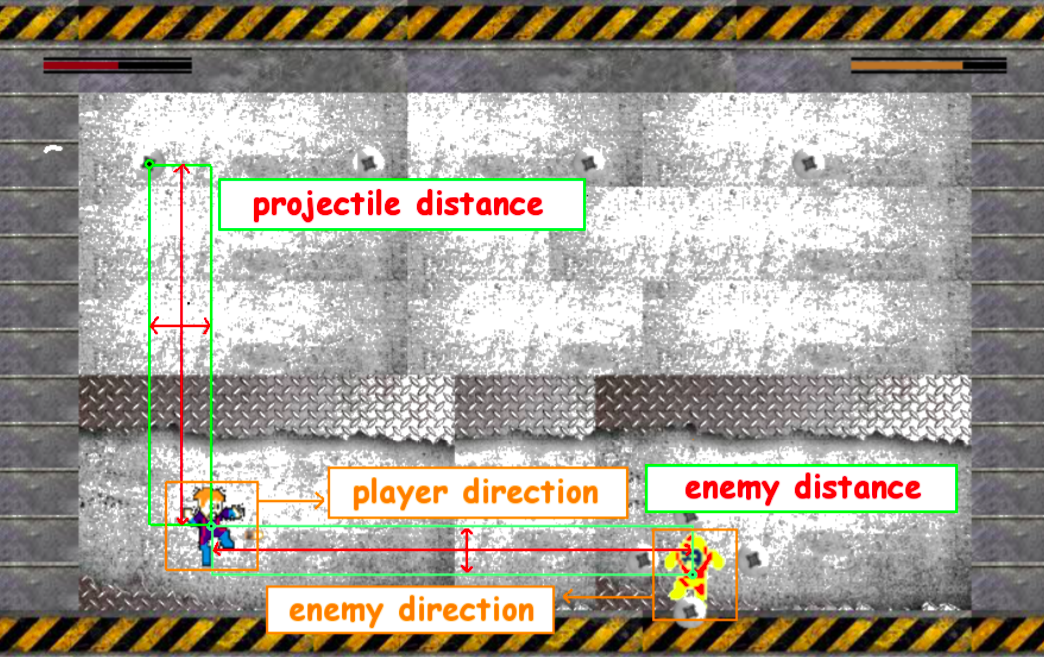
\includegraphics[width=0.9\textwidth]{images/Evoman3.png}
  \end{itemize}
\end{frame}

\begin{frame}{Introduction: Motivation}
  \begin{itemize}
  \item Games are an opportunity to improve our algorithms.
  \item They can be low-cost simulators for interesting problems or topics.
  \item EvoMan was used by a competition at WCCI 2020 (where we placed second). 
  \item We found out that we can greatly improve on the upper bound provided.
  \end{itemize}
\end{frame}

\begin{frame}{Introduction: The difference}
  \begin{itemize}
  \item The initial competition required training with $4$ opponents, and testing on all $8$.
  \item Our approach works better on simply fighting each opponent.
  \item It significantly improves the state of the art results.
  \end{itemize}
\end{frame}

\section{Problem description}
\begin{frame}{Problem description: Evaluation}
  \begin{gather*}
    gain = 100.01 + player\_life - enemy\_life
  \end{gather*}
  \begin{itemize}
  \item Both start with $100$ life points.
  \item the absolute maximum score is $200.01$.
  \item There are $8$ opponents, each with a different strategy.
  \item There are $5$ difficulty levels, each lowering the damage the player does, and increasing the damage the player takes.
  \end{itemize}
\end{frame}

\begin{frame}{Problem description: Agent}
  \begin{itemize}
  \item The game outputs $20$ sensor values, updated each simulation frame.
  \item Each frame, we can perform $5$ actions (e.g. move left, shoot).
    \pause
  \item We chose to place an ANN in this loop.
    \pause
    \item We also remember the past $2$ frames' sensors values, and our past $2$ actions, for a total of $62$ inputs.
  \end{itemize}
\end{frame}

\section{Search Algorithms}

\begin{frame}{Search Algorithms: $2$-stage approach}
  \begin{itemize}
  \item Idea: use an exploratory algorithm to find a good starting point. \pause Tested:
    \begin{itemize}
    \item Random initialisation.
    \item Q-Learning.
    \item Genetic Algorithm (GA).
    \item Particle Swarm Optimisation (PSO).
    \end{itemize}
    \pause
  \item then use an exploitative algorithm to refine that game-playing strategy. We've only used a Proximal Policy Optimisation (PPO) algorithm for this stage.
  \end{itemize}
\end{frame}

\begin{frame}{Search Algorithms: initial comparison}
  \begin{itemize}
  \item No pre-exploration algorithm performed better than random initialisation.
  \item The game is too difficult for basic strategies to constitute the basis for optimal strategies (a misleading / trap function landscape).
  \end{itemize}
\end{frame}

\section{Results}
\begin{frame}{Results: Experiment}
  \begin{itemize}
  \item PPO ran for between $1000$ to $3000$ epochs, per opponent, $30$ repeats for each datapoint.
  \item Time: $1000$ epochs require $\approx 10000000$ ($10M$) Evoman frames.
  \item We ran specialised and generalised PPO models.
  \item Specialised means $8$ models, $1$ for each of the $8$ opponents, $1000$ epochs.
  \item Generalised means $1$ model for all $8$ opponents, $3000$ epochs.
  \end{itemize}
\end{frame}

\begin{frame}{Results: vs the upper bound}
      \begin{table}[htbp]
        \caption{PPO generalised vs PPO specialised vs NEAT specialised, difficulty $= 2$ }
        \begin{center}
            \begin{tabular}{|c|c|c|c|}
                \hline
                \textbf{Opponent}&\textbf{PPO gen.}&\textbf{PPO spec.}&\textbf{NEAT spec.} \\
                \hline
                 1 &  199.54 &  199.67 &  190.01 \\
                 2 &  200.01 &  199.61 &  194.01 \\
                 3 &  194.81 &  199.94 &  180.01 \\
                 4 &  180.61 &  195.95 &  194.01 \\
                 5 &  187.77 &  198.03 &  194.01 \\
                 6 &  174.43 &  199.67 &  173.01 \\
                 7 &  183.07 &  197.73 &  177.01 \\
                 8 &  169.31 &  195.07 &  186.01 \\
                \hline
                \textbf{harmonic mean} & 185.57 & 198.19 & 185.67 \\
                \hline
            \end{tabular}
            \label{PPO generalized vs specialized vs NEAT}
        \end{center}
      \end{table}
\end{frame}

\begin{frame}{Results: all difficulties, generalised}
  \begin{table}[htbp]
        \caption{PPO (generalised) trained against all opponents (Gain)}
        \begin{center}
            \begin{tabular}{|c|c|c|c|c|c|}
                \hline
                \textbf{Opponent}&\multicolumn{5}{|c|}{\textbf{Difficulty}} \\
                \cline{2-6}
                & \textbf{\textit{1}}& \textbf{\textit{2}}& \textbf{\textit{3}} & \textbf{\textit{4}} & \textbf{\textit{5}} \\
                \hline
                 1 &  200.01 &  199.54 &  170.75 &  155.48 &   41.08\\
                 2 &  200.01 &  200.01 &  182.81 &  168.81 &  168.51\\
                 3 &  199.38 &  194.81 &  164.31 &  127.54 &  130.61\\
                 4 &  186.14 &  180.61 &  154.23 &  181.58 &   60.28\\
                 5 &  196.56 &  187.77 &  185.34 &  142.41 &  158.31\\
                 6 &  196.35 &  174.43 &  179.19 &   23.84 &    9.88\\
                 7 &  199.26 &  183.07 &   95.40 &    8.01 &    8.28\\
                 8 &  196.57 &  169.31 &  123.00 &   41.34 &   10.01\\
                \hline
                \textbf{harmonic mean} & 196.68 & 185.57 & 149.57 & 35.76 & 20.89 \\
                \hline
            \end{tabular}
            \label{PPO against all opponents gain}
        \end{center}
    \end{table}
\end{frame}

\begin{frame}{\phantom{Results: all difficulties, generalised}}
  \vspace{-1.1cm}
  \begin{figure}[htbp]
    \centering
    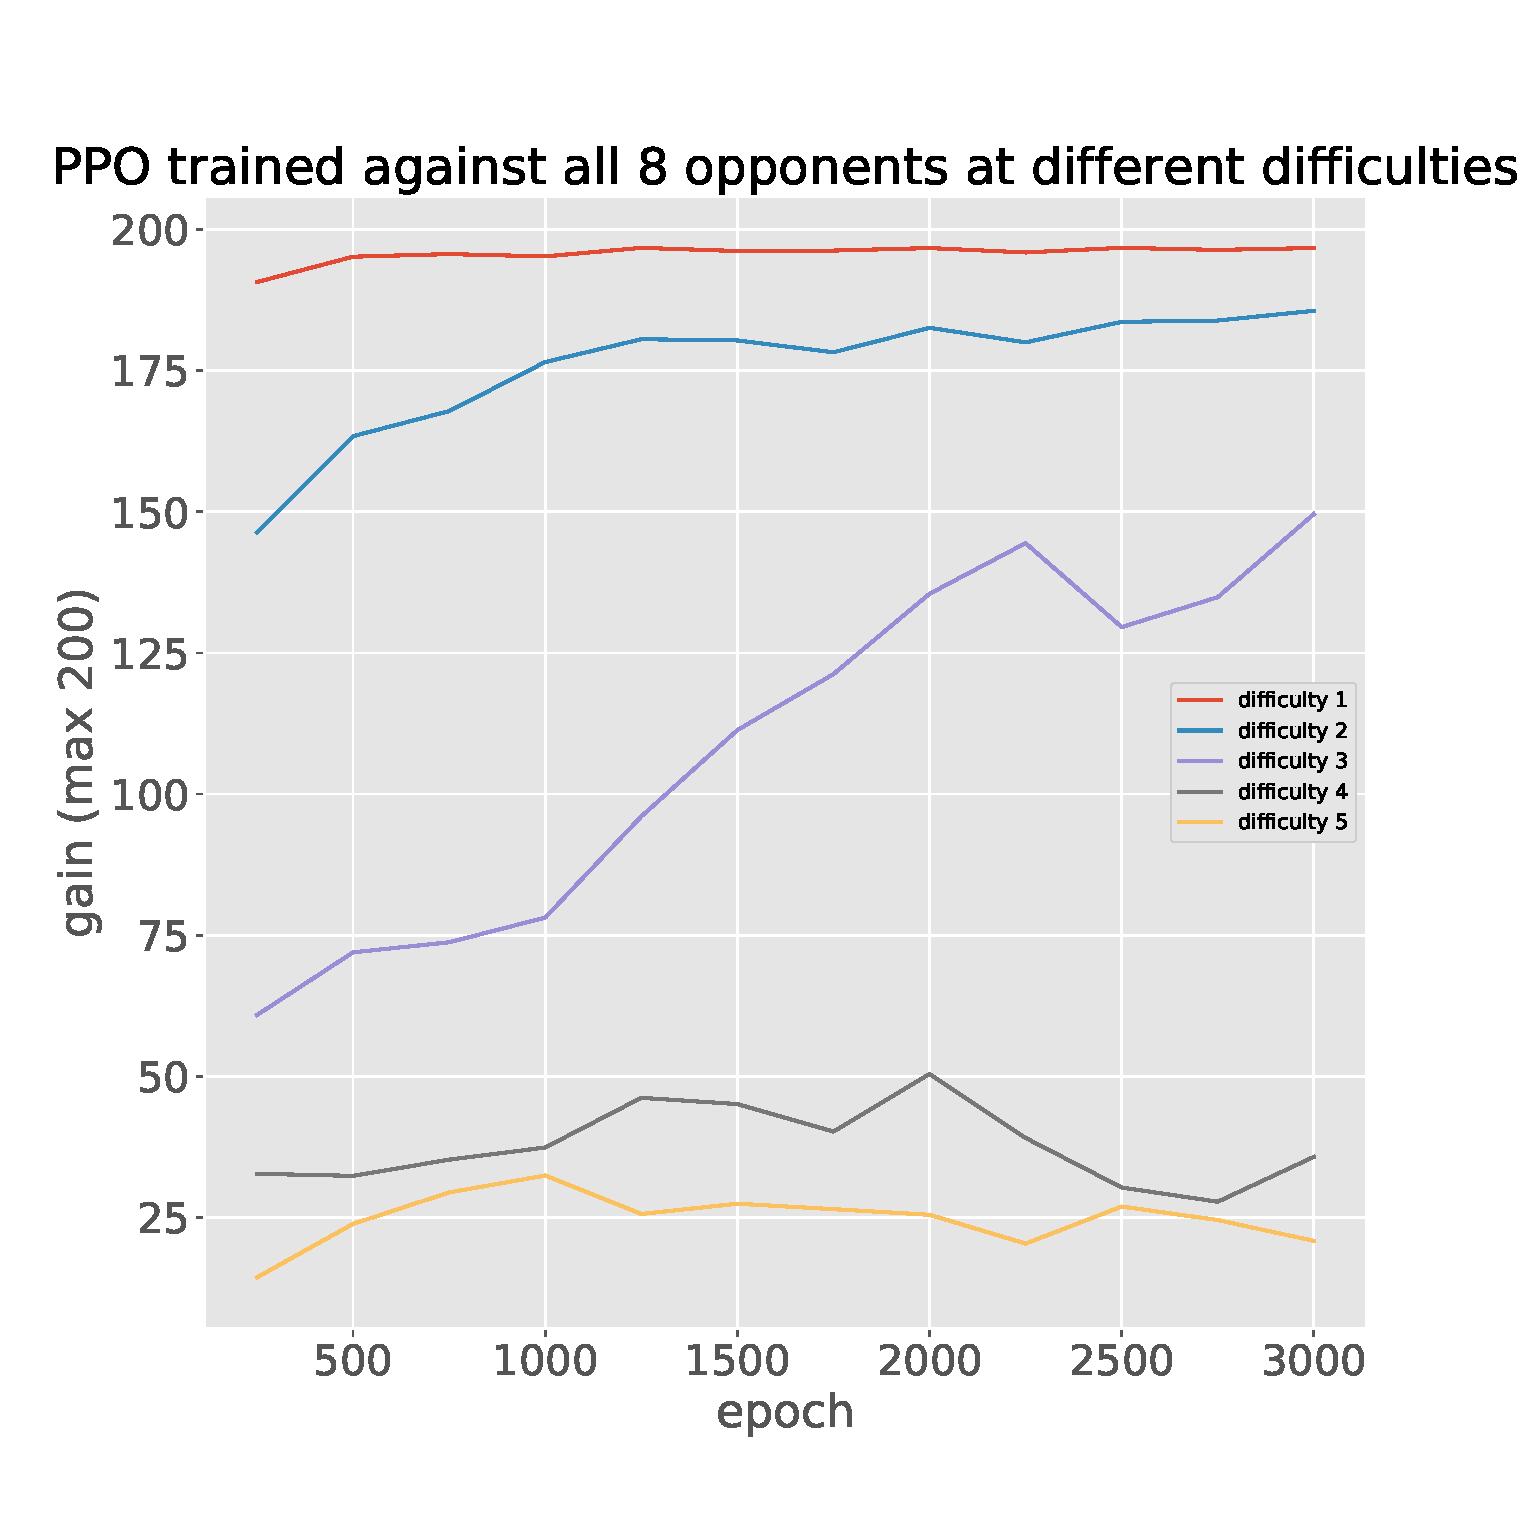
\includegraphics[width=0.9\textwidth]{images/general_harmonic_gain.eps}
    \caption{Gain Evolution for PPO when trained against all 8 opponents.}
    \label{fig:ppo_train_8}
    \end{figure}
\end{frame}

\begin{frame}{Results: all difficulties, specialised}
      \begin{table}[htbp]
      \caption{PPO (specialised), trained $1000$ epochs (gain)}
              \begin{center}
            \begin{tabular}{|c|c|c|c|c|}
                \hline
                \textbf{Opponent} & \multicolumn{4}{|c|}{\textbf{Difficulty}} \\
                \cline{2-5}
                & \textbf{\textit{2}} & \textbf{\textit{3}} & \textbf{\textit{4}} & \textbf{\textit{5}} \\
                \hline
                1                      & 199.68              & 196.51              & 189.21              & 166.01              \\
                2                      & 199.61              & 199.91              & 199.21              & 197.18              \\
                3                      & 199.94              & 199.51              & 147.21              & 72.28               \\
                4                      & 195.95              & 196.14              & 198.81              & 191.23              \\
                5                      & 198.03              & 193.38              & 191.73              & 196.71              \\
                6                      & 199.67              & 195.18              & 196.85              & 198.76              \\
                7                      & 197.73              & 192.45              & 184.85              & 176.01              \\
                8                      & 195.07              & 185.37              & 178.05              & 172.61              \\
                \hline
                \textbf{harmonic mean} & 198.19              & 194.7               & 184.12              & 154.58              \\
                \hline
            \end{tabular}
            \label{Specialized PPO against multiple difficulties (gain)}
        \end{center}
        \end{table}
\end{frame}

\begin{frame}{Results: percentage of games lost}
      \begin{table}[htbp]
        \caption{PPO - percentage of games lost}
        \begin{center}
            \begin{tabular}{|c|c|c|c|c|c|c|c|c|c|}
                \hline
              \textbf{Opp.}&\multicolumn{9}{|c|}{\textbf{Difficulty}} \\
              \cline{2-10}
                           & \multicolumn{5}{|c|}{Generalised} & \multicolumn{4}{|c|}{Specialised} \\
              \cline{2-10}
                & \textbf{\textit{1}}& \textbf{\textit{2}}& \textbf{\textit{3}} & \textbf{\textit{4}} & \textbf{\textit{5}} & \textbf{\textit{2}}& \textbf{\textit{3}} & \textbf{\textit{4}} & \textbf{\textit{5}}\\
                \hline
                 1 &  0 &  0 &     20 &  23.33 &   100 & 0 & 0 & 0     & 13.33 \\
                 2 &  0 &  0 &      0 &      0 &     0 & 0 & 0 & 0     & 0 \\
                 3 &  0 &  0 &      0 &  13.33 &  3.33 & 0 & 0 & 36.67 & 100 \\
                 4 &  0 &  0 &      0 &      0 &    60 & 0 & 0 & 0     & 0 \\
                 5 &  0 &  0 &      0 &      0 &     0 & 0 & 0 & 0     & 0 \\
                 6 &  0 &  0 &      0 &    100 &   100 & 0 & 0 & 0     & 0 \\
                 7 &  0 &  0 &  56.66 &    100 &   100 & 0 & 0 & 0     & 0 \\
                 8 &  0 &  0 &     10 &    100 &   100 & 0 & 0 & 0     & 0 \\
                \hline
            \end{tabular}
            \label{PPO against all opponents games lost}
        \end{center}
    \end{table}
\end{frame}

\begin{frame}{Conclusions}
  \begin{itemize}
  \item We have surpassed the state-of-the-art through an exploitative and time-consuming algorithm.
  \item It is a difficult, misleading problem, since optimal game-playing strategies cannot be easily inferred from suboptimal strategies.
  \item Thus, the cascade method cannot work well. A memetic algorithm (e.g. PSO + PPO) seems feasible.
  \end{itemize}
\end{frame}

%\section{Bibliography}

\begin{thebibliography}{17}

    \bibitem{evoman_competition} Evoman: Game-playing Competition for WCCI 2020, \url{http://pesquisa.ufabc.edu.br/hal/Evoman.html}
    \bibitem{evoman_competition_results} Evoman: Game-playing Competition for WCCI 2020, results \url{http://pesquisa.ufabc.edu.br/hal/Evoman.html#results}
    \bibitem{evoman} Fabricio Olivetti de Franca, Denis Fantinato, Karine Miras, A.E. Eiben and Patricia A. Vargas.
      "EvoMan: Game-playing Competition" arXiv:1912.10445
    \bibitem{karinemiras} de Araújo, Karine da Silva Miras, and Fabrício Olivetti de França.
      "An electronic-game framework for evaluating coevolutionary algorithms." arXiv:1604.00644 (2016).
    \bibitem{neuro} Floreano, D., Dürr, P. \& Mattiussi, C. Neuroevolution: from architectures to learning. Evol. Intel. 1, 47–62 (2008). \url{https://doi.org/10.1007/s12065-007-0002-4}
    \bibitem{capcom} M. MEGA, "Produced by capcom, distributed by capcom, 1987," System: NES.

      \pagebreak
      
    \bibitem{q_learning} Watkins, C.J.C.H., Dayan, P. Q-learning. Machine Learning 8, 279–292 (1992)
    \bibitem{genetic_algorithm} Holland J.H., Genetic Algorithms and Adaptation. Adaptive Control of Ill-Defined Systems, 1984, Volume 16 ISBN 978-1-4684-8943-9
    \bibitem{pso} Kennedy, J.; Eberhart, R. (1995). "Particle Swarm Optimization". Proceedings of IEEE International Conference on Neural Networks. IV. pp. 1942–1948.
    \bibitem{neat} Kenneth O. Stanly; Rist Miikkulainen (2002). "Evolving Neural Networks through Augmenting Topologies". Evolutionary Computation, Volume 10, Issue 2, Summer 2002, p.99-127, \url{https://doi.org/10.1162/106365602320169811}
    \bibitem{ppo} John Schulman, Filip Wolski, Prafulla Dhariwal, Alex Radford, Oleg Klimov (2017) "Proximal Policy Optimization Algorithms", arXiv:1707.06347v2

      \pagebreak
      
    \bibitem{memetic} Moscato, P. (1989). "On Evolution, Search, Optimization, Genetic Algorithms and Martial Arts: Towards Memetic Algorithms". Caltech Concurrent Computation Program (report 826).
    \bibitem{cybenko} Cybenko, G. (1989). "Approximations by superpositions of sigmoidal functions", Mathematics of Control, Signals, and Systems, 2(4), 303–314. doi:10.1007/BF02551274
    \bibitem{nfl} Wolpert, D.H., Macready, W.G. (1997), "No Free Lunch Theorems for Optimization", IEEE Transactions on Evolutionary Computation 1, 67.
    \bibitem{evoman_blog} Karine Miras, Evoman, \url{https://karinemirasblog.wordpress.com/portfolio/evoman/}
    \bibitem{spinningUp} Joshua Achiam, 2018, ``Spinning Up in Deep Reinforcement Learning'' \url{https://github.com/openai/spinningup}
  
\end{thebibliography}



% that's all folks
\end{document}


